\newpage
\section{Analisi statistica FastJson}
Di seguito l'analisi statistica relativa al progetto \textbf{FastJson}.

\subsection{Analisi Statistica Technical Debt}
In \autoref{td_AnalisiFastJson-tipo} possiamo vedere la dimensione del technical debt rispetto alla tipologia di clone. È stato indicato con il valore zero le classi in cui il codice clonato è assente. Questa analisi statistica è confermata dal p-value, ottenuto con il test di Kruskal-Wallis mediante R, che ha un valore inferiore a $2,2 e^{-16}$.
\begin{figure}[htbp]
	\centering
	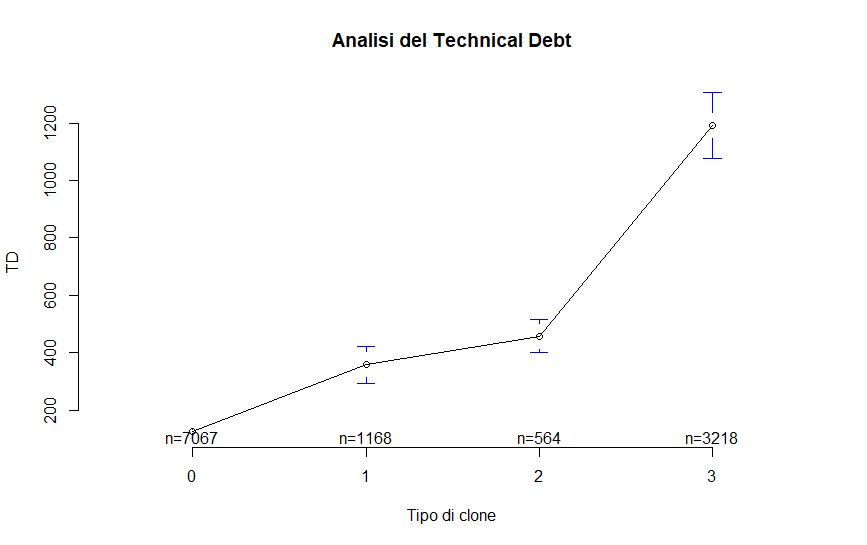
\includegraphics[scale=0.5]{analisi_R/AnalisiFastJson/1-gplot-td-type.png}
\caption{Analisi statistica Technical Debt}
\label{td_AnalisiFastJson-tipo}
\end{figure}


\subsection{Analisi Statistica Code Smells}
In \autoref{codesmell_AnalisiFastJson-tipo} possiamo vedere la quantità di code smells rispetto alla tipologia di clone. È stato indicato con il valore zero le classi in cui il codice clonato è assente. Questa analisi statistica è confermata dal p-value, ottenuto con il test di Kruskal-Wallis mediante R, che ha un valore inferiore a $2,2 e^{-16}$. \newpage
\begin{figure}[htbp]
	\centering
	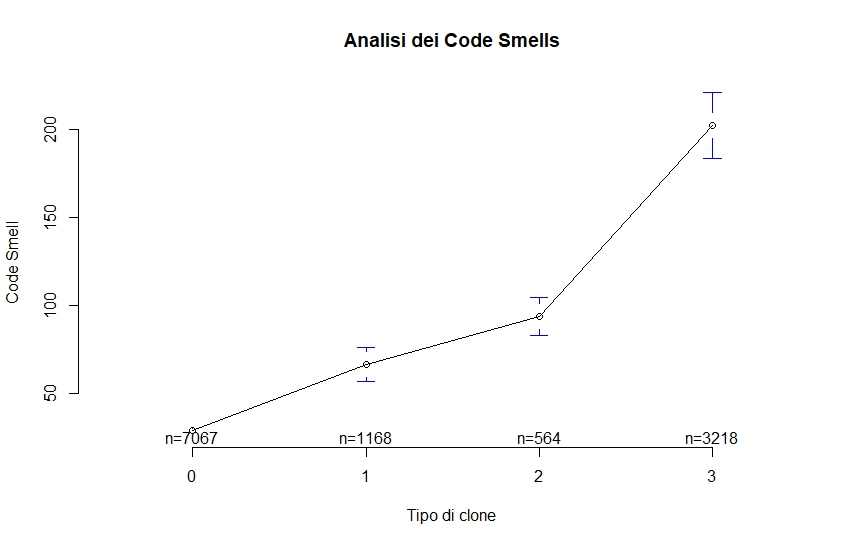
\includegraphics[scale=0.5]{analisi_R/AnalisiFastJson/2-gplot-codesmell-type.png}
\caption{Analisi statistica Code Smell}
\label{codesmell_AnalisiFastJson-tipo}
\end{figure}


\subsection{Analisi Statistica Lunghezza Codice Clonato}
In \autoref{len_AnalisiFastJson-tipo} possiamo vedere la lunghezza del codice clonato (espressa in LOC) rispetto alla tipologia di clone. Questa analisi statistica è confermata dal p-value, ottenuto con il test di Kruskal-Wallis mediante R, che ha un valore inferiore a $6,295e^{-11}$. \newpage
\begin{figure}[htbp]
	\centering
	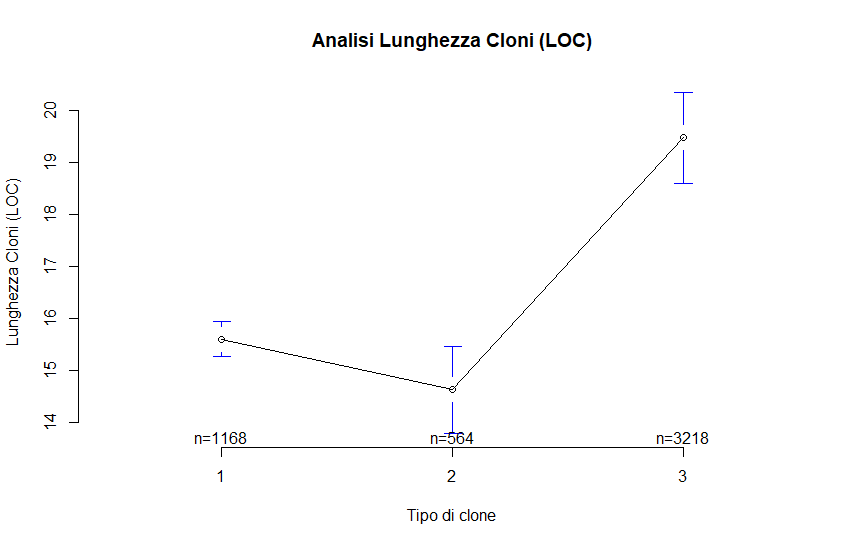
\includegraphics[scale=0.5]{analisi_R/AnalisiFastJson/3-gplot-len-type.png}
\caption{Analisi statistica Lunghezza Codice Clonato }
\label{len_AnalisiFastJson-tipo}
\end{figure}
